\documentclass[13pt, a4paper]{scrartcl}
\usepackage[utf8]{inputenc}
\usepackage{fontenc}
\usepackage{xcolor}
\usepackage{hyperref}
\usepackage[italian]{babel}
\usepackage[inline]{enumitem}
\usepackage{graphicx}
\usepackage{cleveref}

\setlist[enumerate,1]{label=\arabic*}
\setlist[enumerate,2]{label=\theenumi.\arabic*}
\setlist[enumerate,3]{label=\theenumii.\arabic*}

\graphicspath{ {res/} }
\usepackage{url}
\usepackage{acronym}
%\usepackage{natbib}
\usepackage{makeidx}
\usepackage{listings}
\usepackage[square,numbers,sort]{natbib}
\usepackage{tabularx}
\usepackage{float}

% version
\newcommand{\versionmajor}{0}
\newcommand{\versionminor}{1}
\newcommand{\versionpatch}{2}
\newcommand{\version}{\versionmajor.\versionminor.\versionpatch}
\newenvironment{inlinelist}{\begin{enumerate*}[label=\emph{(\roman*)}]}{\end{enumerate*}}
\typeout{Document version: \version}

% acronyms
\acrodef{FC}{Field Calculus}
\acrodef{AC}{Aggregate Computing}
\acrodef{dsl}[DSL]{Domain Specific Language}
\acrodef{ast}[AST]{Abstract Syntax Tree}
\acrodef{xc}[XC]{\emph{eXchange Calculus}}
\acrodef{ci}[CI]{\emph{Continuous Integration}}
\acrodef{cd}[CD]{\emph{Continuous Deployment}}
\acrodef{cicd}[CI/CD]{\ac{ci} and \ac{cd}}
\acrodef{vmc}[VMC]{Vascular Morphogenesis Controller}

\newcommand{\ck}{\emph{Collektive}}

\title{\LARGE
    Un approccio unificante alla programmazione di dispositivi eterogenei nell'edge-cloud continuum \\ \small Prima relazione trimestrale di progetto
}

\author{
   Borsista: \\Angela Cortecchia \\ \small angela.cortecchia@unibo.it
    \and
    Tutor accademico: \\Danilo Pianini \\ \small danilo.pianini@unibo.it
    \and
    Referee CTS GARR: \\Claudio Grandi \\ \small claudio.grandi@bo.infn.it
    \and
    Referee GARR: \\Francesco Lombardi \\ \small francesco.lombardi@garr.it
}

%\date{\small Academic year}
%\makeindex

\begin{document}
\maketitle
\clearpage

%%%%%%%%%%%%%%%%%%%%body%%%%%%%%%%%%%%%%%%%%

\section{Contesto}
\label{sec:context}
In un contesto in cui sono sempre in maggior numero i dispositivi dotati di capacità computazionali,
    che presentano la necessità di un'organizzazione e di un coordinamento tra loro,
    è necessario trovare una soluzione uniforme che permetta di programmare il comportamento e la coordinazione dei dispositivi.

Questi dispositivi possono essere di natura eterogenea, ovvero possono avere architetture e sistemi operativi diversi,
    e possono essere distribuiti in un'area geografica più o meno estesa.
%
La diversa natura di questi dispositivi può portare a problemi di interoperabilità e di comunicazione tra di essi.
%
Possono trovare applicazioni in vari contesti diversi, come ad esempio \emph{smart cities}, \emph{swarm robotics} e \emph{crowd management},
    includendo dispositivi di tipo wearable come smartwatch e smartphone.

La gestione del singolo dispositivo in questi contesti non è banale, possono ad esempio essere presenti $200$ o più dispositivi
    connessi tra loro all'interno di una rete.
%
Gestirli tutti individualmente porterebbe a problemi di scalabilità, manutenibilità ed etereogeneità.

Per questi motivi si vuole passare dall'approccio attuale definito classico con ``device centrico'', ovvero dove il programma è scritto per il singolo dispositivo,
    ad un approccio \emph{collettivo} basato sulla programmazione macroscopica del comportamento dei dispositivi,
    usando tecniche di \emph{\ac{AC}}~\cite{BealIEEEComputer2015}.

\ac{AC} è un paradigma di programmazione che permette di definire un unico comportamento di un insieme di dispositivi,
    definendo l'interazione fra loro.
%
È fondato sull'astrazione del \ac{FC}~\cite{JLAMP2019} che consente di esprimere il comportamento auto-organizzante di reti
    di dispositivi come funzioni riutilizzabili che operano sui campi, dette ``costrutti'' o ``blocchi''.

Per fare ciò, viene sviluppato un \ac{dsl}, denominato \ck{}, basato sui concetti di \ac{AC} e \ac{FC} ed implementato in Kotlin Mulitplatform,
    che permette di scrivere codice in Kotlin e di compilarlo per diverse piattaforme, come JVM, JS, Native, iOS e Android.

\section{Obiettivi raggiunti}\label{sec:obiettivi-raggiunti}

Nella \Cref{fig:timeline} è mostrata la timeline indicativa del progetto, con i task da svolgere e la relativa durata.
%
Al momento ci troviamo tra M3 e M4, in corrispondenza della linea arancione.
%
Di seguito verranno illustrati i task svolti fino ad ora.

\begin{figure}
    \centering
    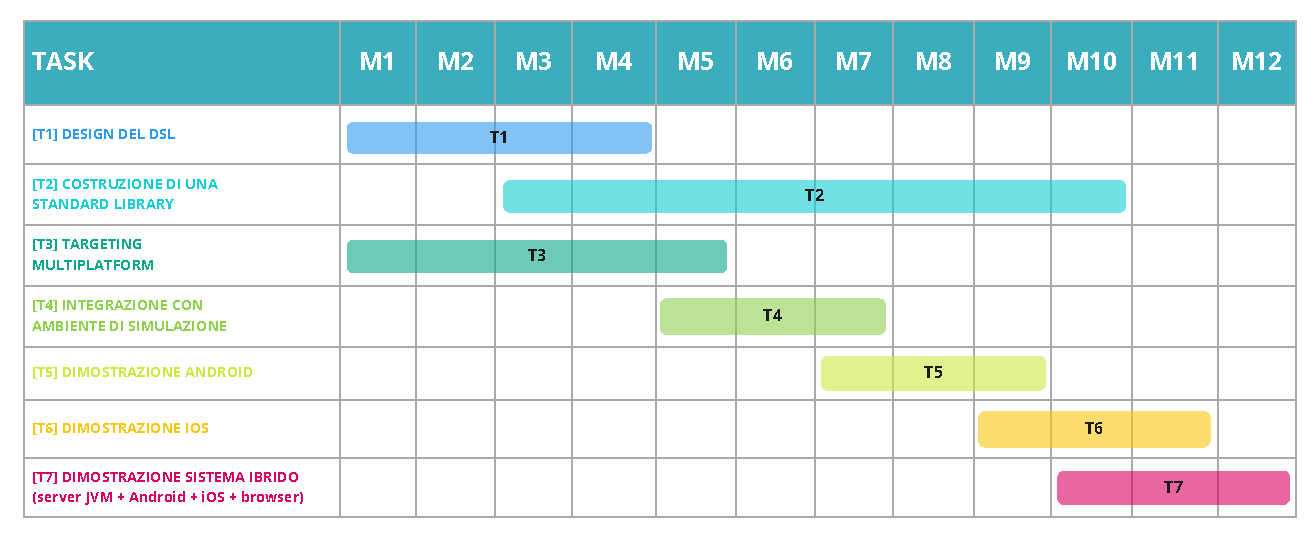
\includegraphics[width=\textwidth]{images/collektive_timeline}
    \caption{Timeline indicativa del progetto.}
    \label{fig:timeline}
\end{figure}

\subsection{Design del DSL [Task T1]}\label{subsec:t1}

\paragraph{DSL}
Per prima cosa è servito capire quali fossero effettivamente i costrutti necessari da inserire all'interno del DSL di \ck{}\footnote{
    Repository con codice open source visitabile al seguente link \url{https://github.com/Collektive/collektive}.
}.
%
Tra i vari approcci proposti per l'implementazione del \ac{FC}, è stato scelto di utilizzare \ac{xc}~\cite{AudritoCDSV24}.
%
\ac{xc} è un linguaggio di programmazione sperimentale per lo sviluppo di sistemi distribuiti omogenei che segue le astrazioni
    di \ac{AC}.

Astraendo da concorrenza, perdita di messaggi, protocollo di comunicazione di rete e fallimenti dei nodi,
    \ac{xc} permette di definire un modello di calcolo distribuito che si basa su un insieme di regole di trasformazione
    che operano sui campi computazionali,
    rivelandosi un modello di calcolo ideale per il progetto.

\ac{xc} è basato su una primitiva di comunicazione che permette di scambiare messaggi tra dispositivi --\emph{exchange}--,
    con l'aspetto cruciale che può inviare messaggi con valori diversi a seconda del vicino, consentendo un'interazione
    personalizzata tra essi.
%
Utilizzando questo costrutto è possibile implementare gli altri costrutti del \ac{FC}.

Identificato dunque il costrutto di base del \ac{dsl}, è stato possibile implementare altri costrutti per la comuncazione
    con peculiarità diverse, quali:
\begin{itemize}
    \item \emph{exchange}: per lo scambio di messaggi personalizzati tra dispositivi, restituendo al programma lo stesso
        valore che viene inviato ai vicini;
    \item \emph{exchanging}: come \emph{exchange}, ma restituisce un valore diverso da quello inviato;
    \item \emph{share}: implementato in termini di \emph{exchange}, permette di condividere un valore ai vicini, indistintamente
        dal destinatario, restituendo al programma il valore condiviso;
    \item \emph{sharing}: come \emph{share}, ma restituisce un valore diverso da quello condiviso;
    \item \emph{repeat}: costrutto del \ac{FC} che permette di modellare l'evoluzione nel tempo dello stato del dispositivo.
        In quanto non è necessaria comunicazione con i vicini, non è stato implementato in termini di \emph{exchange}.;
    \item \emph{repeating}: come \emph{repeat}, ma restituisce un valore diverso da quello restituito dall'iterazione precedente.
    \item \emph{neighboring}: costrutto del \ac{FC} che permette di accedere ai valori dei vicii e inviare loro informazioni,
        permettendo così di modellare l'evoluzione dell'informazione nello spazio.
        Implementato sia in termini di exchange che non, con differenze in termini di performance.
\end{itemize}

L'utilizzo di \ac{xc} porta un'innovazione aggiuntiva, in quanto al momento lo stato dell'arte non prevede l'implementazione di
    questa primitiva all'interno di un \ac{dsl}.


\paragraph{Compiler Plugin}

Per permettere una corretta comunicazione dei dispositivi, esiste il concetto di ``allineamento''.
%
La semantica del \ac{FC} è definita compositiva ed i messaggi scambiati tra vicini vengono automaticamente abbinati
    allo stesso costrutto del programma, determinato da un processo chiamato allineamento.
%
Ogni costrutto genera un ``export'', un valore di dati da inviare ai vicini, creando quindi un enriched \ac{ast} fino a quel costrutto.
%
Questi export vengono raccolti in un messaggio da trasmettere ai vicini, che può essere modellato come
    un albero ordinato di valori ottenuti durante la valutazione di ogni sottoespressione del programma.

Il meccanismo di allineamento assicura che ogni sotto-programma di un dispositivo sia abbinato al corrispondente dei vicini,
    seguendo un percorso identico nell'albero di valutazione,
    permettendo cosi di far comunicare i dispositivi allineati tra di loro.

Per fare ciò, è stato implementato un plugin per il compilatore di Kotlin, che si occupa di annotare le funzioni visitate
    durante la valutazione del programma, in modo da poter creare un path di esecuzione che permetta di allineare i dispositivi
    tra di loro.

\subsection{Costruzione di una standard library [Task T2]}\label{subsec:task-t2-[costruzione-di-una-standard-library]}

Per capire quali fossero le principali funzionalità necessarie in una standard library,
è stato deciso di implementare una generalizzazione di un noto algoritmo in letteratura, chiamato \ac{vmc}~\cite{ZahadatHS17},
applicando un approccio basato su \ac{AC} e \ac{FC}, utilizzando il \ac{dsl} di \ck{}.

\ac{vmc} permette di modellare la crescita di strutture artificiali nel tempo, ispirandosi alla morfogenesi delle piante.
%
L'algoritmo si basa su un modello di distribuzione delle risorse in strutture ad albero,
    dove i rami competono per le risorse per crescere, in base al successo ottenuto come input da sensori nell'ambiente.

Implementando l'algoritmo con \ck{}, è stato possibile identificare le funzionalità chiave da cui partire per costruire la standard library,
    confrontando il lavoro con la libreria di base di Protelis,
    un linguaggio di programmazione per sistemi auto-organizzanti basato su \ac{FC},

Dal lavoro ottenuto con lo sviluppo dell'algoritmo,
    è stato possibile sottoportare un articolo alla conferenza ``\emph{Autonomic Computing and Self-Organizing Systems}'' (ACSOS) 2024
    \footnote{\url{https://2024.acsos.org}},
    intitolato ``\emph{An Aggregate Vascular Morphogenesis Controller for Engineered Self-Organising Spatial Structures}'',
    che propone un modello alternativo al \ac{vmc} proposto in letteratura,
    sviluppato con \ck{}.
%
Per poter validare il lavoro svolto, è stata necessaria l'integrazione con un simulatore,
    per controllare la correttezza del sistema e comprenderne il comportamento in scenari diversi.
%
Ciò ha portato dunque ad una prima versione rudimentale del task T4, ovvero l'integrazione con un ambiente di simulazione.
%
Come ambiente di simulazione, è stato deciso di integrare \ck{} con \emph{Alchemist}~\cite{PianiniJOS2013},
    un meta-simulatore per pervasive computing e sistemi distribuiti,
    basato su astrazioni generali che possono essere mappate a casi d'uso specifici.
%
Data l'integrazione con \emph{Alchemist}, è stato possibile creare alcuni esperimenti nell'ambito di \ac{vmc},
    sempre presentati ad ACSOS 2024, che hanno permesso di validare il lavoro svolto \footnote{
    Gli esperimenti sono open source ed è possibile visionarli al seguente link \url{https://github.com/angelacorte/vmc-experiments}.
}.

\subsection{Targeting multiplatform [Task T3]}\label{subsec:task-t3-[targeting-multiplatform]}
Per quanto riguarda il targeting delle varie piattaforme,
    sono stati implementati i test usando la libreria \emph{Kotest},
    una libreria di testing per Kotlin che permette di scrivere test in modo conciso e leggibile.
%
I test vengono eseguiti automaticamente ad ogni push sul repository, grazie all'integrazione con GitHub Actions in modalità \ac{cicd}.

Il \ac{dsl} è dunque testato con esiti positivi su JVM, JS, Nativo ed emulatore di iOS, watchOS e tvOS.
%
Al momento non sono ancora presenti i test per Android, che verranno sviluppati in seguito,
    non si prevedono però particolari problemi di compatibilità in quanto Android è basato su JVM.

\section{Prossimi obiettivi}\label{sec:prossimi-obiettivi}

%completamento t1 t3
%implementazione standard library in contrapposizione a quella di protelis -francia
%ulteriori sviluppi di t4
%allineamento debug-friendly
%investigare integrazione con pulverization

Come obiettivi per i prossimi tre mesi di lavoro, ovvero nella \Cref{fig:timeline} tra M6 e M7,
    si prevede di completare il task T1, ovvero la progettazione del \ac{dsl},
    ed il task T3, ovvero il targeting multiplatform,
    aspirando all'effettivo testing del \ac{dsl} su Android e piattaforme iOS fisiche.

Gli sviluppi dell'integrazione con l'ambiente di simulazione (task T4) e della standard library (task T2) verranno portati
    avanti, con l'obiettivo di implementare funzionalità più complesse.

Inoltre, si prevede di implementare un meccanismo di allineamento più debug-friendly,
    per permettere una migliore comprensione del comportamento dei dispositivi durante l'esecuzione del programma.

Come attuale lavoro in svolgimento c'è anche la stesura di un altro articolo, che verrà presentato alla conferenza
    ``\emph{Distributed Simulation in the Space Domain}'' (DS-RT) 2024
    \footnote{\url{http://ds-rt.com/2024/}},
    per il quale verranno sviluppate simulazioni di programmi implementati con \ck{} in un ambiente di simulazione distribuito.

Infine, non si esclude la possibilità di una collaborazione all'interno del gruppo di ricerca UniBo con colleghi che stanno sviluppando
    ricerche sull'approccio ``polverizzazione''~\cite{fi12110203}:
    un approccio utilizzato per progettare il comportamento adattivo distribuito per Sistemi Cibernetici-Fisici (CPS) su larga scala,
    suddividendo il comportamento complessivo del sistema in piccoli pezzi di calcolo gestibili strettamente legati a sensori, attuatori e componenti vicini.
%
Questa collaborazione potrebbe portare a una posticipazione dei task inerenti alle demo, ma permetterebbe di sviluppare
    un approccio più generale e flessibile per la programmazione di dispositivi eterogenei nell'edge-cloud continuum.

%%%%%%%%%%%%%%%%%%%%end%%%%%%%%%%%%%%%%%%%%

% add more ....

\bibliographystyle{plain}
\bibliography{bibliography}

\end{document}